% !TEX root = ./0.main.tex
在本节中,我们将阐述问题并详细介绍拟议的框架,并说明我们的框架与代表性的现有方法之间的区别。

\begin{table}
  \centering
  \caption{\label{tab:notation} 符号表.}
%   \small
%   \renewcommand{\arraystretch}{1.2}
  \begin{tabular}{c|p{2.55in}}
    \hline \hline
    \textbf{Notation} & \textbf{Description} \\
    \hline
    $u$ & 一个用户 \\
    $i$ & 一个项 \\
    $e$ & 一个交互 \\
    $\mathcal{U}$ & 用户集 \\
    $\mathcal{I}$ & 项集 \\
    % $\mathcal{E}$ & a user's sequence \\
    $\mathcal{I}_u$ & 用户的测试项集 $u$ \\
    % $\mathcal{D}$ & the set of training samples \\
    % $\mathcal{D}^{+/-}$ & the set of positive/negative training samples \\
    $d$ & 用户/项目嵌入的维度 \\
    $K$ & 兴趣嵌入的数量 \\
    $N$ & 候选项目数 \\
    $\mathbf{V}_u$ & 用户$u$ 的兴趣嵌入矩阵 \\
    $\delta(\cdot)$ & 指示函数 \\
    % $\mathbf{e}_i$ & the vector of primary capsule $i$ \\
    % $\mathbf{v}_j$ & the vector of interest capsule $j$ \\
    % $b_{ij}, c_{ij}$ & coupling coefficients of dynamic routing \\
    % $\mathbf{W}$ & transformation matrix \\
    \hline \hline
  \end{tabular}
\end{table}

\subsection{问题表述}
%~\cite{he2016fusing,hidasi2015session,rendle2010factorizing,smirnova2017contextual,tang2018personalized,tang2019towards}
% We formulate the \textit{sequential recommendation} problem as a sequence prediction problem. 
%recommend a set of items to each user that the user may be most interested in.
假设我们有一组用户 $u\in \mathcal{U}$ 和一组项目 $i\in \mathcal{I}$. 对于每个用户,我们都有一系列用户历史行为 $(e^{(u)}_{1}, e^{(u)}_{2}, \cdots, e^{(u)}_{n})$,按出现时间排序。$e^{(u)}_{t}$ 记录用户交互的第 $t^{th}$ 项。给定历史交互,\textit{顺序推荐}问题指预测用户可能会与之交互的下一个项目。
表~\ref{tab:notation} 中概述了用到的符号.

实际上,由于对延迟和性能的严格要求,工业推荐系统通常包括两个阶段,即匹配阶段和排名阶段。匹配阶段对应于检索前N个候选项目,而排名阶段用于按更精确的分数对候选项目进行排序。本文主要关注在匹配阶段提高有效性。在本节的以下部分中,我们将介绍可控制的多兴趣框架,并说明该框架对于\textit{顺序推荐}问题的重要性. % The overview of our models can be seen in Figure~\ref{fig:capsule}.

\begin{figure*}
    \centering
    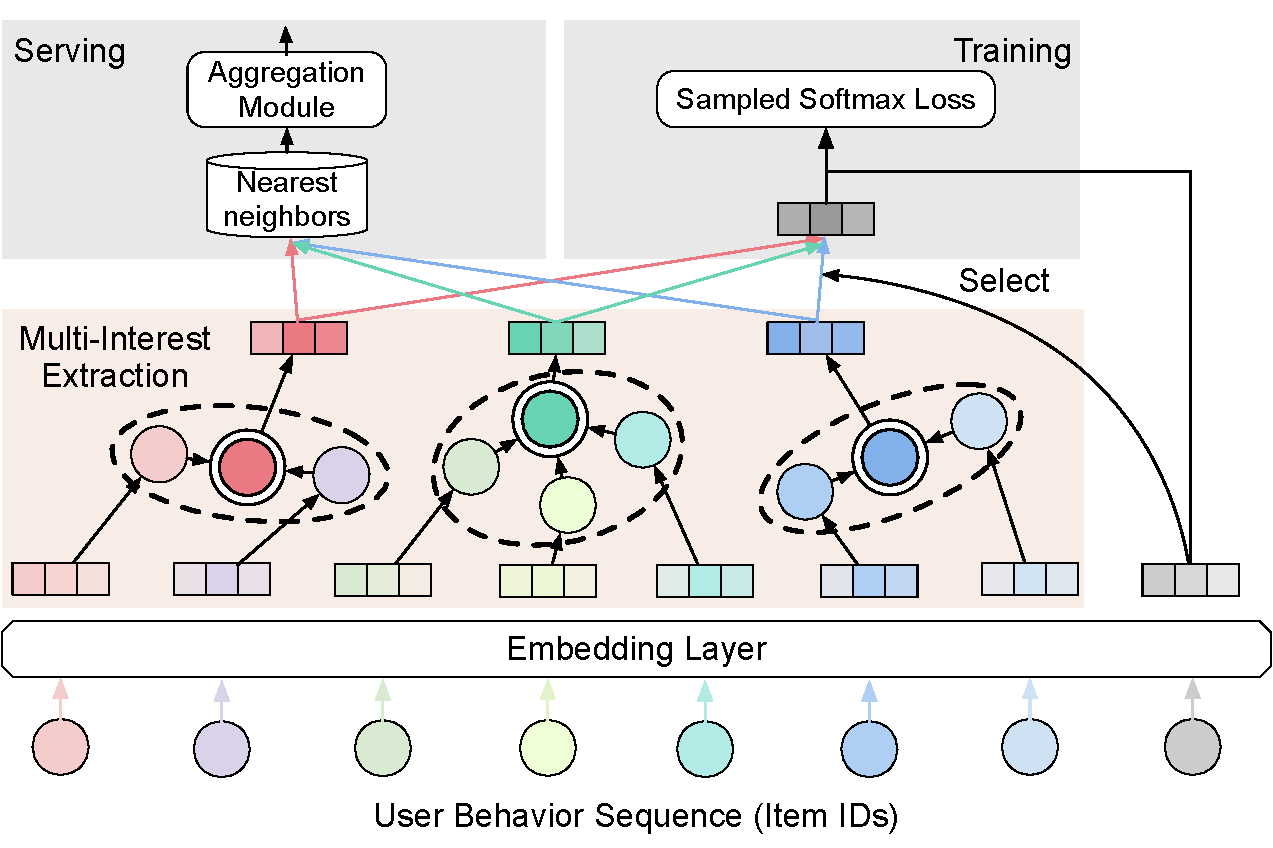
\includegraphics[width=0.8\textwidth]{figures/multi-interest-framework.pdf}
    \caption{顺序推荐模型的概述。我们模型的输入是用户行为序列,其中包含项ID的列表。该项目ID被送入嵌入层,并转化到该项目的嵌入。 兴趣嵌入是通过多兴趣提取模块生成的,然后可用于模型训练和服务。对于模型训练,将选择与目标嵌入最接近的兴趣嵌入来计算采样的softmax损失。为了提供服务,每个兴趣嵌入都将独立检索前N个最近的项目,然后将其馈入聚合模块。聚合模块通过可控制的过程来生成总体前N个项目,从而平衡推荐准确性和多样性。 }
    \label{fig:capsule_matching}
\end{figure*}

\subsection{多兴趣框架}
作为工业推荐系统的项目池通常由数百万甚至数十亿的项目,匹配阶段起着推荐系统至关重要的作用。 具体而言,匹配模型首先根据用户的历史行为来计算用户嵌入,然后基于用户嵌入为每个用户检索一组候选项目。借助快速K近邻算法(KNN)从大型项目池中选择最接近的项目以为每个用户生成候选集,我们主要集中在用户嵌入的计算上。换句话说,根据用户历史行为计算出的用户嵌入质量是匹配阶段的决定性因素。

现有的匹配模型通常使用RNN\cite{hidasi2015session,wu2017recurrent}为用户计算嵌入,但是大多数模型仅为每个用户生成一个嵌入向量。由于现实世界中的客户通常会考虑几种商品,而这些商品通常用于不同的用途,并且类别差异很大,因此,这种单一嵌入的方式缺乏足够的表达能力。 现实世界中客户的这种行为突显了需要使用多个向量来表示多重兴趣的重要性。基于这些考虑,我们为顺序推荐提出了一个多兴趣框架。我们框架的输入是用户行为序列,其中包含项目ID的列表,这些ID代表用户按时间顺序与商品的交互。商品ID被馈送到嵌入层,并转换为商品嵌入。多兴趣提取模块接收项目嵌入,并为每个用户生成多个兴趣。

%Interest capsules are generated through the dynamic routing method and can be then used for model training and online serving.

% RNN-based models~\cite{hidasi2015session,wu2017recurrent} are widely used in sequential recommendation. These models are effective for short-term user sequences~\cite{tang2019towards} but cannot capture long-term user interests from user sequences. 
To build a multi-interest extraction module, there are many optional methods. In this paper, we explore two methods, dynamic routing method and self-attentive method, as our multi-interest extraction module. Our framework using a dynamic routing method or self-attentive method is named as \model-DR or \model-SA, respectively. 

\vpara{Dynamic Routing.}
%\zc{The motivation to exploit multi-interest network as the long-range model should be highlighted.}
We utilize a dynamic routing method as a multi-interest extraction module for user behavior sequences. The item embeddings of the user sequence can be viewed as primary capsules, and the multiple user interests can be seen as interest capsules. We use the dynamic routing method from CapsNet~\cite{sabour2017dynamic}. 
We briefly introduce dynamic routing for computing vector inputs and outputs of capsules. A capsule is a group of neurons whose activity vectors represent the instantiation parameters of a specific type of entity such as an object or an object part~\cite{sabour2017dynamic}. The length of the output vector of a capsule represents the probability that the entity represented by the capsule is in the current input. Let $\mathbf{e}_i$ be the capsule $i$ of the primary layer. We then give the computation of the capsule $j$ of the next layer based on primary capsules. 
%How to calculate capsules $\mathbf{v}_j$ of the output layer? 
We first compute the prediction vector as
\begin{equation}
    \hat{\mathbf{e}}_{j|i}=\mathbf{W}_{ij} \mathbf{e}_{i},
\end{equation}
where $\mathbf{W}_{ij}$ is a transformation matrix. Then the total input to the capsule $j$ is the weighted sum over all prediction vectors $\hat{\mathbf{e}}_{j|i}$ as
\begin{equation}
        \mathbf{s}_j = \sum_i c_{ij} \hat{\mathbf{e}}_{j|i},
\end{equation}
where $c_{ij}$ are the coupling coefficients that are determined by the iterative dynamic routing process. The coupling coefficients between capsule $i$ and all the capsules in the next layer should sum to 1. We use ``routing softmax'' to calculate the coupling coefficients using initial logits $b_{ij}$ as
\begin{equation}
    c_{ij}=\frac{\exp(b_{ij})}{\sum_k \exp(b_{ik})},
\end{equation}
where $b_{ij}$ represents the log prior probability that capsule $i$ should be coupled to capsule $j$. A non-linear "squashing" function~\cite{sabour2017dynamic} is proposed to ensure short vectors to get shrunk to almost zero length and long vectors to get shrunk to a length slightly below 1. Then the vector of of capsule $j$ is computed by
\begin{equation}
    \label{eqn:squash}
    \mathbf{v}_j = \operatorname{squash}(\mathbf{s}_j) =  \frac{\|\mathbf{s}_j\|^2}{1+\|\mathbf{s}_j\|^2} \frac{\mathbf{s}_j}{\|\mathbf{s}_j\|},
\end{equation}
where $\mathbf{s}_j$ is the total input of capsule $j$. To calculate the output capsules $\mathbf{v}_j$, we need to calculate the probability distribution based on the inner production of $\mathbf{v}_j$ and $\mathbf{e}_i$. The calculation of $\mathbf{v}_j$ relies on itself; thus, dynamic routing method is proposed to solve this problem. The whole dynamic routing process is listed in Algorithm~\ref{algo:dynamic_routing}. The output interest capsules of the user $u$ are then formed as a matrix $\mathbf{V}_u=[\mathbf{v}_1, ..., \mathbf{v}_K] \in \mathbb{R}^{d\times K}$ for downstream tasks.

% In order to ensure the diversity between interest capsules, we introduce a penalty term similar with \cite{lin2017structured}.

% \begin{equation}
%     P = \sum_{u\in \mathcal{U}}||\mathbf{V}_u \mathbf{V}_u^T-\mathbf{I}||_F^2
% \end{equation}
% where $||\cdot||_F$ denotes the Frobenius norm of a matrix. The penalty term $P$ will be multiplied by a coefficient and then added to the original loss (binary cross entropy loss or sampled softmax loss).

\begin{algorithm}[t]
	\caption{Dynamic Routing \label{algo:dynamic_routing}}
	\KwIn{primary capsules $\mathbf{e}_i$, iteration times $r$, number of interest capsules $K$}
	\KwOut{interest capsules $\{\mathbf{v}_j, j=1,...,K\}$}
	for each primary capsule $i$ and interest capsule $j$: initialize $b_{ij} = 0$. \\
    \For{$iter = 1,\cdots,r$} {
        for each primary capsule $i$: $\mathbf{c}_i = \operatorname{softmax}(\mathbf{b}_{i})$.\\
        for each interest capsule $j$: $\mathbf{s}_j = \sum_{i} c_{ij}\mathbf{W}_{ij}\mathbf{e}_i$.\\%\hat{\mathbf{e}_{j|i}}$. \\

        for each interest capsule $j$: $\mathbf{v}_j = \operatorname{squash}(\mathbf{s}_j)$. \\

        for each primary capsule $i$ and interest capsule $j$: $b_{ij} = b_{ij}+ \mathbf{v}_j^\top \mathbf{W}_{ij}\mathbf{e}_i$.
    }
    \Return{$\{\mathbf{v}_j, j=1,...,K\}$}
\end{algorithm}


\vpara{Self-Attentive Method.} 
The self-attentive method~\cite{lin2017structured} can also be applied to our multi-interest extraction module. 
Given the embeddings of user behaviors, $\mathbf{H}\in \mathbb{R}^{d\times n}$, where $n$ is the length of the user sequence, we use the self-attention mechanism to obtain a vector of weights $\mathbf{a} \in \mathbb{R}^{n}$:
\begin{equation}
    \mathbf{a} = \operatorname{softmax}(\mathbf{w}_{2}^\top \operatorname{tanh}(\mathbf{W}_{1} \mathbf{H}))^\top,
\end{equation}
\noindent where $\mathbf{w}_{2}$ and $\mathbf{W}_{1}$ are trainable parameters with size $d_a$ and $d_a \times d$, respectively. The superscript $\top$ denotes the transpose of the vector or the matrix. The vector $\mathbf{a}$ with size $n$ represents the attention weight of user behaviors. When we sum up the embeddings of user behaviors according to the attention weight, we can obtain a vector representation $\mathbf{v}_u = \mathbf{H} \mathbf{a}$ for the user. For the self-attentive method to make use of the order of user sequences, we add trainable positional embeddings~\cite{vaswani2017attention} to the input embeddings. The positional embeddings have the same dimension $d$ as the item embeddings and the two can be directly summed. 

This vector representation focuses on and reflects a specific interest of the user $u$. To represent the overall interests of the user, we need multiple $\mathbf{v}_u$ from the user behaviors that focus on different interests. Thus we need to perform multiple times of attention. We extend the $\mathbf{w}_{2}$ into a $d_a$-by-$K$ matrix as $\mathbf{W}_{2}$. Then the attention vector $\mathbf{a}$ becomes an attention matrix $\mathbf{A}$ as
\begin{equation}
    \mathbf{A} = \operatorname{softmax}(\mathbf{W}_{2}^\top \operatorname{tanh}(\mathbf{W}_{1} \mathbf{H}))^\top.
\end{equation}

The final matrix of user interests $\mathbf{V}_u$ can be computed by
\begin{equation}
    \label{eqn:sa}
    \mathbf{V}_u = \mathbf{H} \mathbf{A}.
\end{equation}



\vpara{Model Training.}
After computing the interest embeddings from user behaviors through the multi-interest extraction module, we use an \textit{argmax} operator to choose a corresponding user embedding vector for a target item $i$:

\begin{equation}
    \label{eqn:argmax}
    \begin{aligned}
        % \mathbf{v}_u & = \operatorname{Attention}(\mathbf{e}_i, \mathbf{V}_u, \mathbf{V}_u) \\
        % & = \mathbf{V}_u \operatorname{softmax}(\mathbf{V}_u^\top \mathbf{e}_i),
        \mathbf{v}_u = \mathbf{V}_u[:, \operatorname{argmax}(\mathbf{V}_u^\top \mathbf{e}_i)],
    \end{aligned}
\end{equation}
where $\mathbf{e}_i$ denotes the embedding of the target item $i$, and $\mathbf{V}_u$ is the matrix formed by user interest embeddings. %The function $\operatorname{pow}$ is the element-wise exponential function and $p$ is a hyperparameter which controls the attention distribution. 

Given a training sample $(u,i)$ with the user embedding $\mathbf{v}_u$ and the item embedding $\mathbf{e}_i$, we can compute the likelihood of the user $u$ interacting with the item $i$ as

\begin{equation}
    \label{eqn:likelihood}
    P_\theta(i|u) = \frac{\exp(\mathbf{v}_u^\top \mathbf{e}_i)}{\sum_{k\in\mathcal{I}}\exp(\mathbf{v}_u^\top \mathbf{e}_k)}.
\end{equation}

The objective function of our model is to minimize the following negative log-likelihood

\begin{equation}
    \label{eqn:loss}
    loss = \sum_{u\in \mathcal{U}} \sum_{i\in \mathcal{I}_u} -\log P_\theta(i|u).
\end{equation}

The sum operator of equation (\ref{eqn:likelihood}) is computationally expensive; thus, we use a sampled softmax technique~\cite{jean2014using, covington2016deep} to train our model.

\vpara{Online Serving.}
For online serving, we use our multi-interest extraction module to compute multiple interests for each user. Each interest vector of a user can independently retrieve top-N items from the large-scale item pool by the nearest neighbor library such as Faiss~\cite{JDH17}. The items retrieved by multiple interests are fed into an aggregation module to determine the overall item candidates. Finally, the items with higher ranking scores will be recommended for users.


% \subsection{Multi-Interest Extraction Module}


\begin{algorithm}[t]
	\caption{Greedy Inference \label{algo:greedy_infer}}
	\KwIn{Candidate item set $\mathcal{M}$, number of output items $N$}
	\KwOut{Output item set $\mathcal{S}$}
	$\mathcal{S} = \varnothing$ \\
    \For{$iter = 1,\cdots,N$} {
        $j = \operatorname{argmax}_{i \in \mathcal{M} \backslash \mathcal{S}} \left( f(u, i) + \lambda \sum_{k \in \mathcal{S}} g(i,k) \right)$ \\
        $\mathcal{S} = \mathcal{S} \cup \{j\}$
    }
    \Return{$\mathcal{S}$}
\end{algorithm}

\subsection{Aggregation Module}
After the multi-interest extraction module, we obtain multiple interest embeddings for each user based on his/her past behavior. Each interest embedding can independently retrieve top-N items based on the inner production proximity. But how to aggregate these items from different interests to obtain the overall top-N items? A basic and straightforward way is to merge and filter the items based on their inner production proximity with user interests, which can be formalized as
\begin{equation}
    f(u,i) = \max_{1\leq k\leq K}(\mathbf{e}_i^\top \mathbf{v}_u^{(k)}),
\end{equation}
where $\mathbf{v}_u^{(k)}$ is the $k$-th interest embedding of the user $u$. This is an effective method for the aggregation process to maximize the recommendation accuracy. However, it is not all about the accuracy of current recommender systems. People are more likely to be recommended with something new or something diverse. 
The problem can be formulated in the following. Given a set $\mathcal{M}$ with $K\cdot N$ items retrieved from $K$ interests of a user $u$, find a set $\mathcal{S}$ with $N$ items such that a pre-defined value function is maximized. Our framework uses a controllable procedure to solve this problem. We use the following value function $Q(u,S)$ to balance the accuracy and diversity of the recommendation by a controllable factor $\lambda \geq 0$,
\begin{equation}
    Q(u,\mathcal{S}) = \sum_{i\in \mathcal{S}} f(u,i) + \lambda \sum_{i\in \mathcal{S}} \sum_{j\in \mathcal{S}} g(i,j).
\end{equation}
\noindent Here $g(i,j)$ is a diversity or dissimilarity function such as
\begin{equation}
    g(i,j) = \delta(\operatorname{CATE}(i) \neq \operatorname{CATE}(j)).
\end{equation}
where $\operatorname{CATE}(i)$ means the category of item $i$ and $\delta(\cdot)$ is an indicator function. 
For the most accurate case, i.e., $\lambda=0$, we just use the above straightforward method to obtain the overall items. For the most diverse case, i.e., $\lambda=\infty$, the controllable module finds the most diverse items for users. We study the controllable factor in the Section~\ref{sec:control_study}. We propose a greedy inference algorithm to approximately maximize the value function $Q(u,S)$, which is listed in the Algorithm~\ref{algo:greedy_infer}.


\subsection{Connections with Existing Models}
We make a comparison between our model and existing models. 

\vpara{MIMN.}
MIMN~\cite{pi2019practice}, a recent representative work for the ranking stage of recommendation, uses memory networks to capture user interests from long sequential behavior data. Both MIMN and our model target at the multiple interests of users. For very long sequential behaviors, a memory-based architecture may also be insufficient to capture the long-term interests of users. Compared with MIMN, our model utilizes the multi-interest extraction module to leverage multiple interests of users instead of a complicated memory network with memory utilization regularization and memory induction unit. 

\vpara{MIND.}
MIND~\cite{li2019multi}, a recent representative work for the matching stage of recommendation, proposes a Behavior-to-Interest (B2I) dynamic routing for adaptively aggregating user's behaviors into interest representation vectors. Compared with MIND, \model-DR follows the original dynamic routing method used by CapsNet~\cite{sabour2017dynamic}, which can capture the sequential information of user behaviors. Our framework also explores a self-attentive method for multi-interest extraction. Moreover, our framework utilizes a controllable aggregation module to balance the recommendation accuracy and diversity based on users' multiple interests. 

% Specifically, MIND uses fully shared transformation matrices, i.e., $\mathbf{W}_{ij}=\mathbf{W}$. In this situation, B2I dynamic routing ignores the item positions and considers the item sequence as an item set. However, the item positions are important for the sequential recommendation. 
%In this situation, the logits $b_{ij}$ cannot be initialized as zeros and are randomly initialized as Gaussian distribution for each batch, which may impact the semantics of capsules. 
% Our method uses partially shared transformation matrices, i.e., $\mathbf{W}_{ij}=\mathbf{W}_j$. 
%% vim: formatoptions=
